\chapter{Introduction}


When I began this PhD in the autumn of 2021, the research community was still marveling at OpenAI's GPT-3 \citep{brown2020gpt3}, a language model with \textbf{175 billion parameters}—a number so vast it felt, at the time, like a ceiling. This impression of scale was even more striking when compared with the \textbf{86 billion neurons} in the adult human brain \citep{azevedo2009neurons}. To many, this parallel symbolized the astonishing pace at which artificial systems appeared to be encroaching on biological complexity.

Yet in the short span of four years, that sense of awe has been recontextualized. \textbf{GPT-4}, though not officially disclosed, is widely estimated to contain \textbf{around 1.8 trillion parameters}, while Google's \textbf{Gemini Ultra} has been reported at roughly \textbf{1.5 trillion}. These figures mark an \emph{order-of-magnitude leap} from GPT-3 and reflect a broader trend: the frontier of large-scale language models is rapidly expanding—both in scale and in sophistication.

This expansion has been accompanied by clear gains in capability. Tasks once viewed as aspirational—such as reasoning over long contexts, synthesizing code, or interpreting multi-step instructions—have become tractable for these large models. Performance is typically benchmarked on standard evaluations like MMLU \citep{hendrycks2021mmlu}, BIG-bench \citep{srivastava2023bigbench}, and HellaSwag \citep{zellers2019hellaswag}, where state-of-the-art models have seen rapid gains since 2021.


\begin{figure}[htbp]
    \centering
    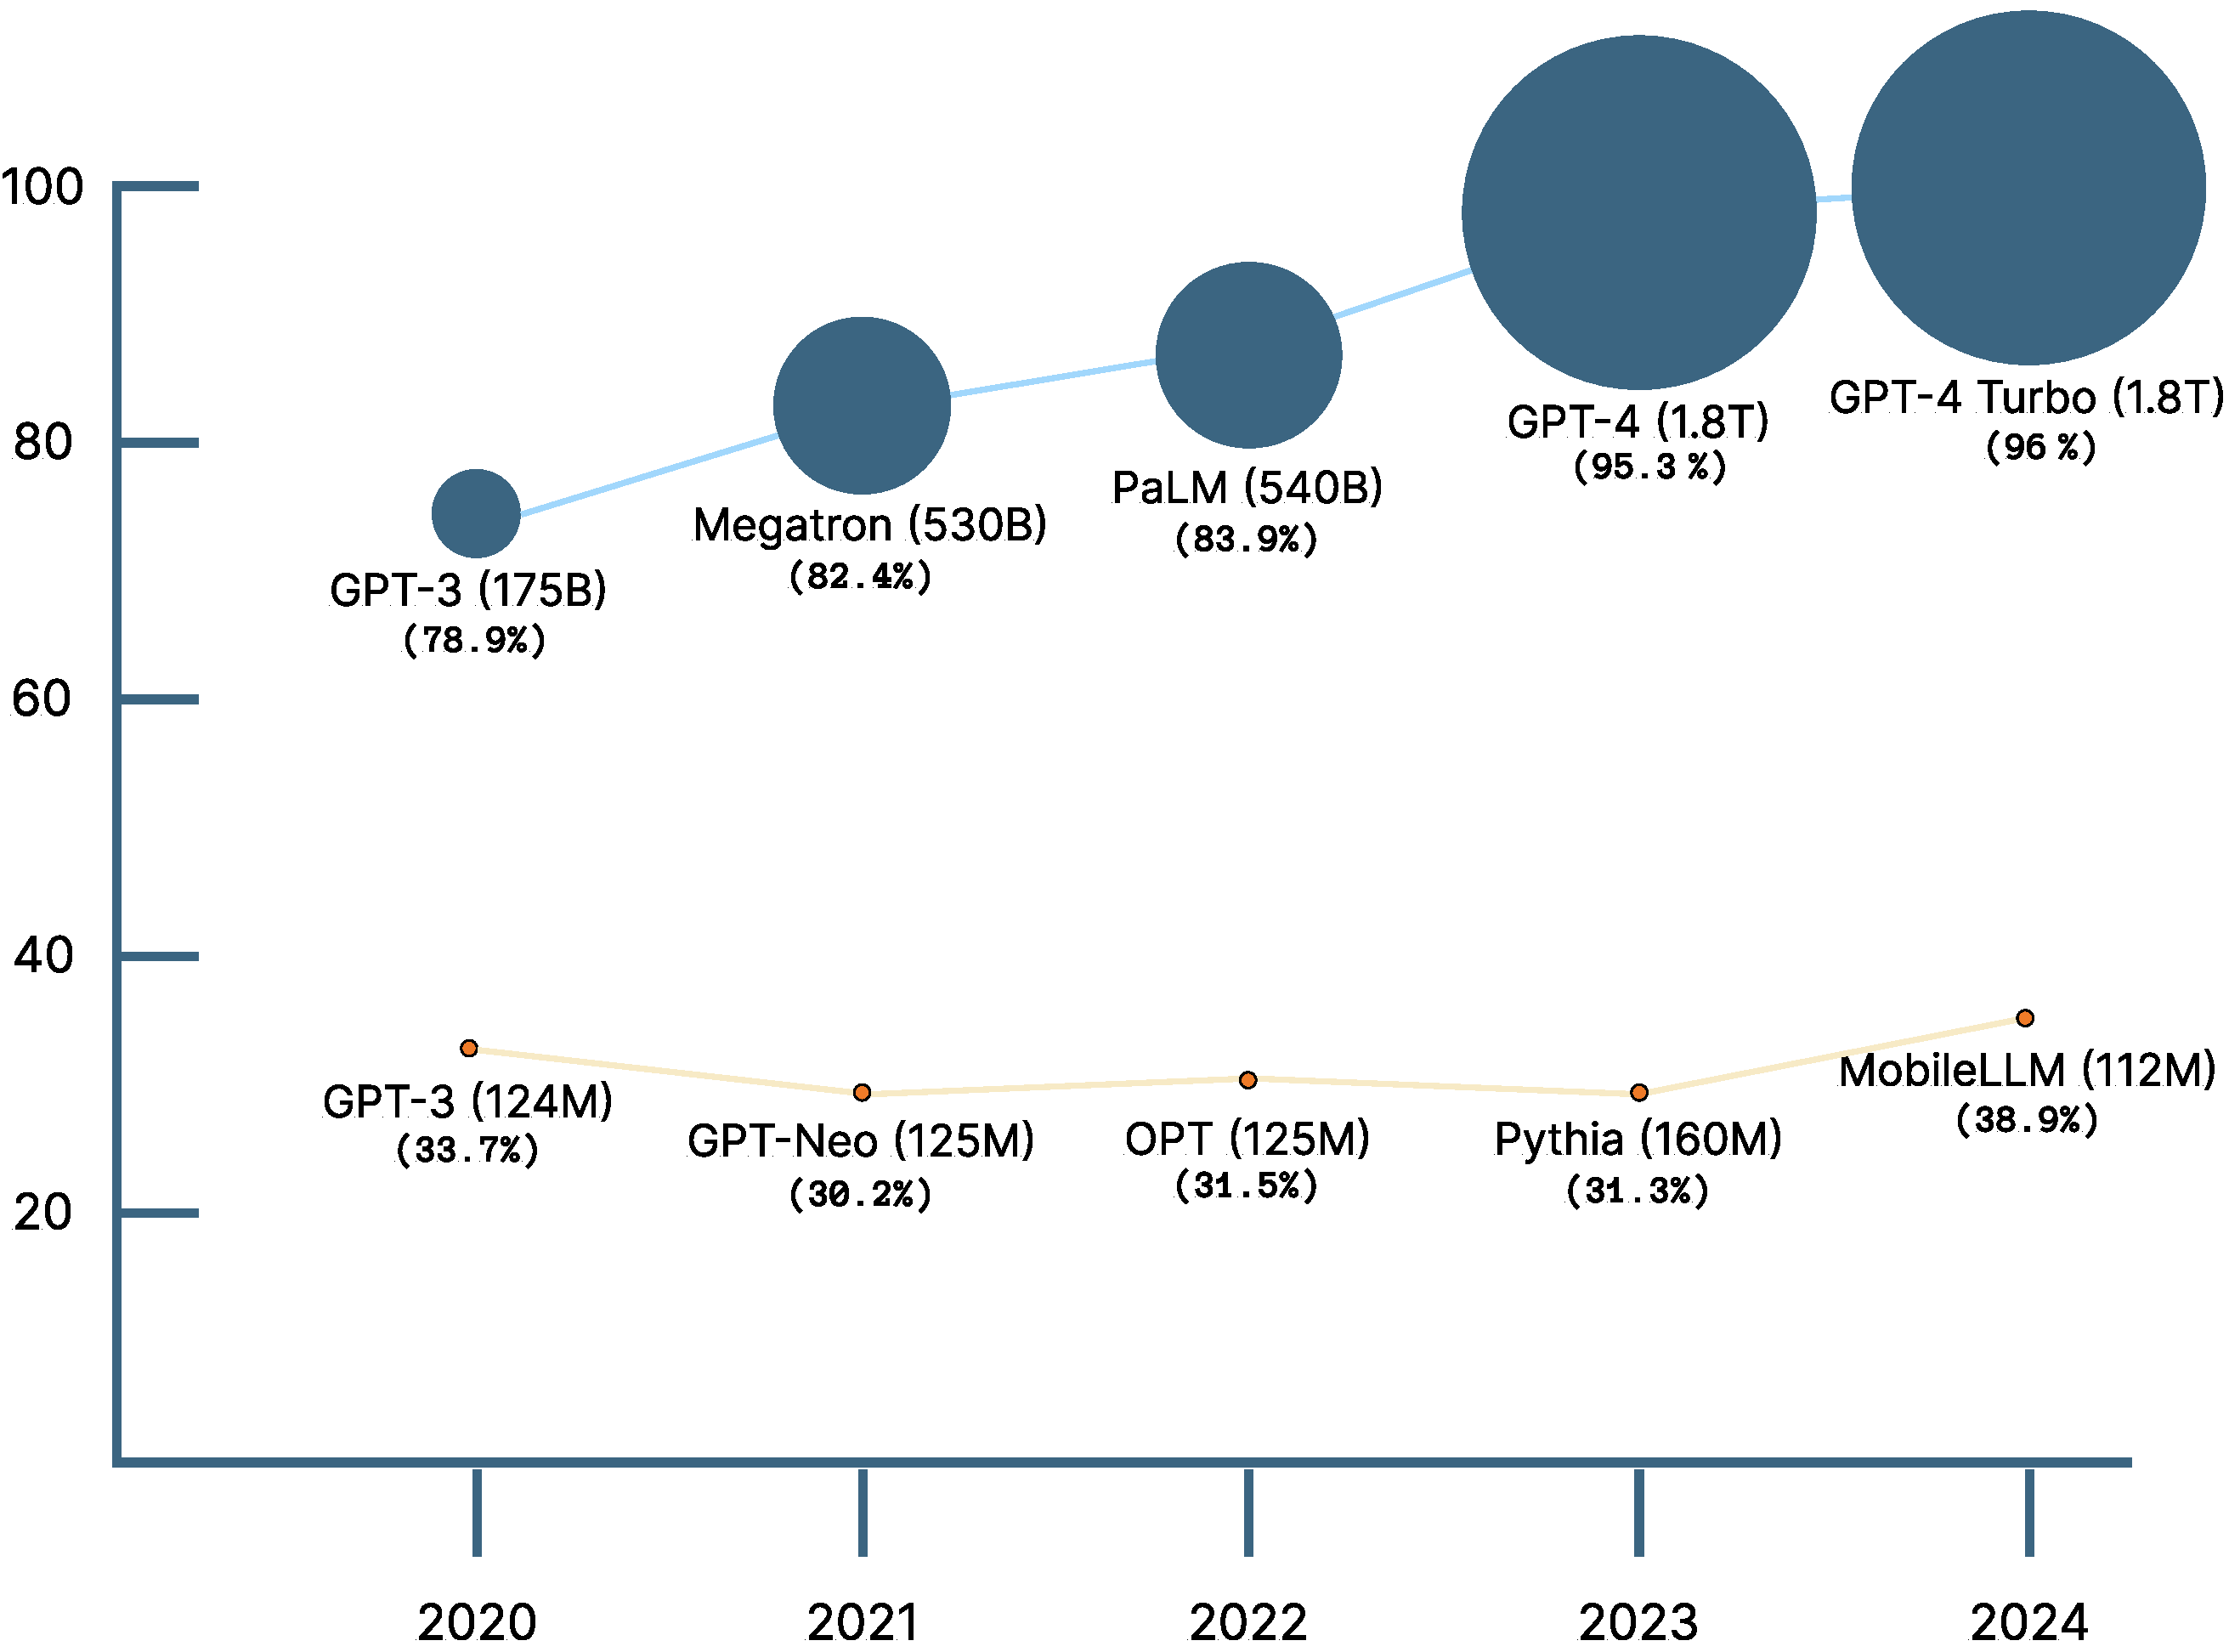
\includegraphics[width=0.8\textwidth]{chapters/introduction/figures/lm_performance_comparison.pdf}
    \caption{Performance of small and large language models on the HellaSwag dataset over time.}
    \label{fig:model_size_vs_performance}
\end{figure}

However, this progress has been \emph{uneven}. In 2020, the best performing model on the HellaSwag dataset (a task that requires reasoning over long contexts) was GPT-3, achieving a score of 78.9\%. In 2024, the best performing model was a novel variant of GPT-4, achieving a nearly perfect score of 96\%. On one hand, this is a testament to the rapid progress of large language models. However, the improvement in performance only tells one half of the story. Between 2020 and 2024, the number of parameters in the best performing model has increased by a factor of 14.5x (from 124M to 1.8T). 

Another problem with studying small language models is that the definition of a `small' language model keeps changing. When GPT-3 was released, 8 versions of the model were released, from GPT-3 Small (125M) to the largest variant (175B) that became commonly referred to as GPT-3. By late 2024, language modeling suites marketed as `small' typically, such as the set of Phi-4 models, contain 14B parameters, with a 3.8B variant labeled as `tiny'.


As we can see in \cref{fig:model_size_vs_performance}, much of the gain in performance has been due to scaling up the model size. If we hold the size of a model constant, we see that smaller models perform the same on task while large models keep getting larger and getting better. Can we claim to making progress if the techniques we are developing are only working because we are using larger and larger models?


While large models have seen dramatic improvements, \textbf{smaller language models have advanced more modestly}, with persistent gaps in performance, generalization, and stability. 

This discrepancy raises a key research question:

\begin{quote}
\textbf{Can small language models be trained more effectively—not simply scaled down, but optimized through strategic methods to unlock their full potential?}
\end{quote}


This dissertation is driven by that question. While large models continue to push boundaries, \textbf{small models remain essential} for practical deployment. They offer advantages in compute efficiency, privacy, customization for domain-specific data, and environmental sustainability. They also support better interpretability and accessibility for researchers with limited resources.

% The final point on interpretability should maybe be along the lines of us being able to more easily interpret why a model is doing something or aligning it

\section*{Research Objectives}

The central aim of this thesis is to investigate how small language models can be trained \emph{more efficiently}, improving their performance through principled strategies rather than brute-force scaling. This goal is pursued along two complementary research threads:


\subsection*{1. Cognitive Inspiration}

The first approach draws insight from the most efficient language learner we know: the human brain. Humans acquire language with \emph{far less data} than large language models. A thirteen-year-old child may have been exposed to approximately \textbf{100 million words}, whereas today's models are trained on over \textbf{10 billion tokens}. This contrast motivates the integration of cognitive principles—such as curriculum learning, syntactic generalization, and frequency-independent representation—into model training.

\begin{quote}
\textbf{To what extent can we take inspiration from the human brain when designing learning paradigms for smaller models?} 
\end{quote}

\subsection*{2. Analytical Examination}

The second approach is analytical. It focuses on building tools and frameworks to observe and understand the \emph{learning dynamics} of small language models. This includes examining how models learn, where training breaks down, and why certain configurations fail to converge. Fine-grained diagnostics of weights, gradients, and activation patterns help identify and mitigate inefficiencies in small model training.

\section*{Thesis Overview}

This thesis is organized into two parts, reflecting the two research threads:

\subsection*{Part I: Cognitive Insights for Efficient Training (Chapters 2–3)}

\begin{itemize}
    \item \textbf{Chapter 2:} \emph{Curriculum Learning for Infant-Inspired Model Building}  
    explores curriculum strategies inspired by human language acquisition, using the BabyLM Challenge's strict 10-million-word cap as a testbed for evaluating data-efficient learning.

    \item \textbf{Chapter 3:} \emph{Mitigating Frequency Bias and Anisotropy in Language Model Pre-Training with Syntactic Smoothing}  
    introduces a novel technique to improve the representation of infrequent tokens by distributing learning signals through syntactic similarity, reducing reliance on frequency and improving robustness.
\end{itemize}

\subsection*{Part II: An Analytical Lens on Learning Dynamics (Chapters 4–5)}

\begin{itemize}
    \item \textbf{Chapter 4:} \emph{Tending Towards Stability: Convergence Challenges in Small Language Models}  
    investigates why small models often saturate during training. Using the Pythia model suite, it analyzes activation patterns, parameter rank, and convergence behavior.

    \item \textbf{Chapter 5:} \emph{Pico: A Lightweight Framework for Studying Language Model Learning Dynamics}  
    presents Pico, a modular framework for transparent training and in-depth analysis of learning dynamics, enabling reproducible experiments with small models.
\end{itemize}

\subsection*{Chapter 6: Concluding Remarks}

Summarizes the core findings of this thesis and outlines promising directions for future research.

\section*{Contributions}

This work contributes to the field by:

\begin{enumerate}
    \item Providing a theoretical and empirical basis for cognitive strategies that reduce the data and compute required to train language models.
    \item Introducing novel methods—such as syntactic smoothing and structured curricula—for improving small model generalization.
    \item Developing analysis tools and frameworks to diagnose and optimize training dynamics in small-scale models.
\end{enumerate}

Together, these contributions aim to support a more \textbf{accessible, efficient, and sustainable future} for language modeling—particularly for researchers and developers working under real-world constraints.
